\documentclass[25pt, a0paper, portrait]{tikzposter}
\usepackage[utf8]{inputenc}
\usepackage{authblk}

\usepackage[backend=biber,style=authoryear,sorting=ynt]{biblatex}
\AtEveryBibitem{%
  \clearfield{issn} % Remove issn
  \clearfield{doi} % Remove doi
  \clearfield{title} % Remove title

  \ifentrytype{online}{}{% Remove url except for @online
    \clearfield{url}
  }
}
\addbibresource{document.bib}

\makeatletter
\renewcommand\maketitle{\AB@maketitle} % revert \maketitle to its old definition
%\renewcommand\AB@affilsepx{\quad\protect\Affilfont} % put affiliations into one line
\makeatother
\renewcommand\Affilfont{\small} % set font for affiliations

\title{\parbox{\linewidth}{\centering Finite-T neutron capture study of Sn isotopes}}

\author[1]{\Large A. C. Berceanu}
\author[1, 2]{\Large Y. F. Niu}
\author[1]{\Large Y. Xu}

\affil[1]{ELI-NP, “Horia Hulubei” National Institute for Physics and Nuclear Engineering,
30 Reactorului Street, RO-077125, Bucharest-Magurele, Romania}
\affil[2]{School of Nuclear Science and Technology, Lanzhou University, Lanzhou 730000, China}

% todo: remove
\usepackage{blindtext}
%\usepackage{comment}

\usetheme{Board}


\begin{document}

\maketitle
\node[anchor=west] at (TP@title.west) {
\includegraphics[width=10cm]{images/eli_logo.pdf}};
\node[anchor=east] at (TP@title.east) {
\includegraphics[width=10cm]{images/ifin_logo.pdf}};
%\node[anchor=west,yshift=-2cm] at (TP@title.west) {
\includegraphics[width=10cm]{images/eli_logo.pdf}};
%\node[anchor=east,yshift=-1cm] at (TP@title.east) {
\includegraphics[width=10cm]{images/eli_logo.pdf}};


%\note[targetoffsetx=-9cm, targetoffsety=-6.5cm, width=0.5\linewidth]{e-mail \texttt{welcome@overleaf.com}}

\begin{columns}
    \column{0.5}

    \block{Abstract}
    {The r-process nucleosynthesis is responsible for the creation of about half of
    the atomic nuclei heavier than iron, under extreme density and temperature
    conditions. As such, the temperature dependence of neutron capture cross
    sections and rates is important for determining the reaction dynamics. As shown
    by the sensitivity study in~\cite{Mumpower2016}, neutron capture dynamics
    on Sn isotopes are very important for r-process study.  So in this work, we
    study the effect of finite temperature on the neutron-capture cross sections and
    rates of even-even tin isotopes, with neutron numbers between 76 and 96.  We
    compute the E1 dipole strengths, for both zero and finite temperature, using
    relativistic Hartree-Bogoliubov (RHB) + quasiparticle random phase approximation
    (QRPA) and finite-temperature relativistic mean-field (FTRMF) +
    finite-temperature random-phase approximation (FTRPA), respectively. We use the
    TALYS code for computing the corresponding cross sections, replacing its default
    E1 dipole data with ours.  We find out the main effect of temperature is to
    increase the low-lying E1 strength, and as a result, the neutron capture cross
    sections are increased several times up to the temperature of 2 MeV.}

    \block{More text}{Text and more text}

	\block{E1 $\gamma$ strength functions (I)}
    {
        \begin{tikzfigure}
            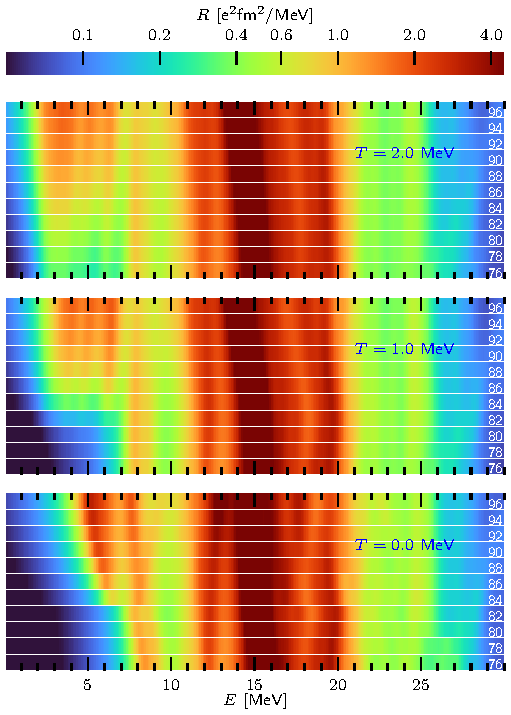
\includegraphics[width=0.4\textwidth]{images/colormesh.pdf}
        \end{tikzfigure}
    }

    \block{References}{
        \printbibliography[heading=none]}


    \column{0.5}

    \block{Cross section}{
        \begin{tikzfigure}
            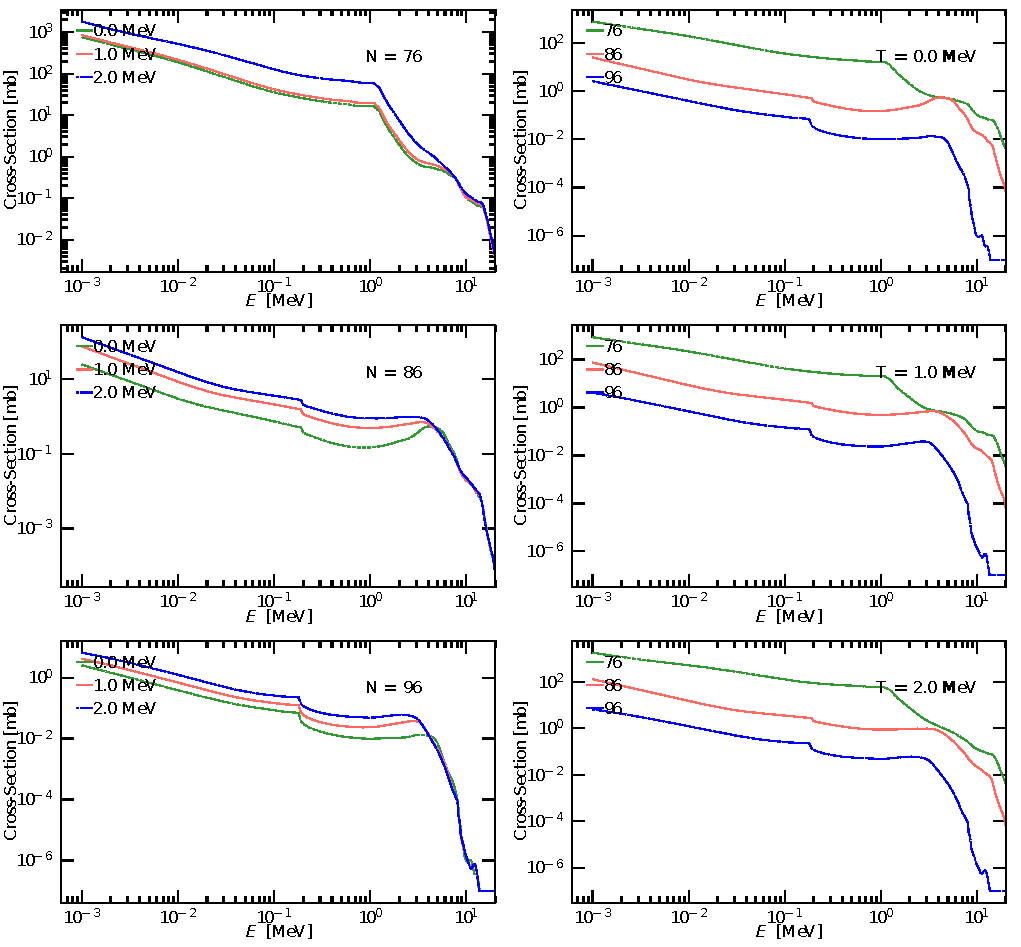
\includegraphics[width=0.4\textwidth]{images/cross_section.pdf}
        \end{tikzfigure}
    }

    \block{Neutron capture rate}{
        \begin{tikzfigure}
            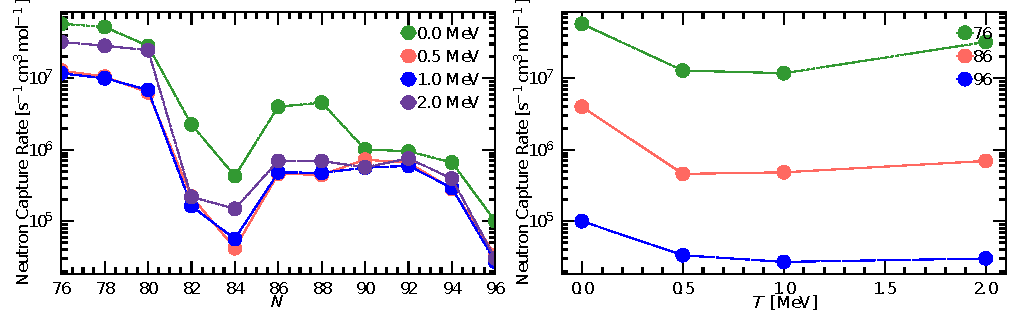
\includegraphics[width=0.4\textwidth]{images/capture_rate.pdf}
        \end{tikzfigure}
    }

	\block{E1 $\gamma$ strength functions (II)}
    {
        \begin{tikzfigure}
            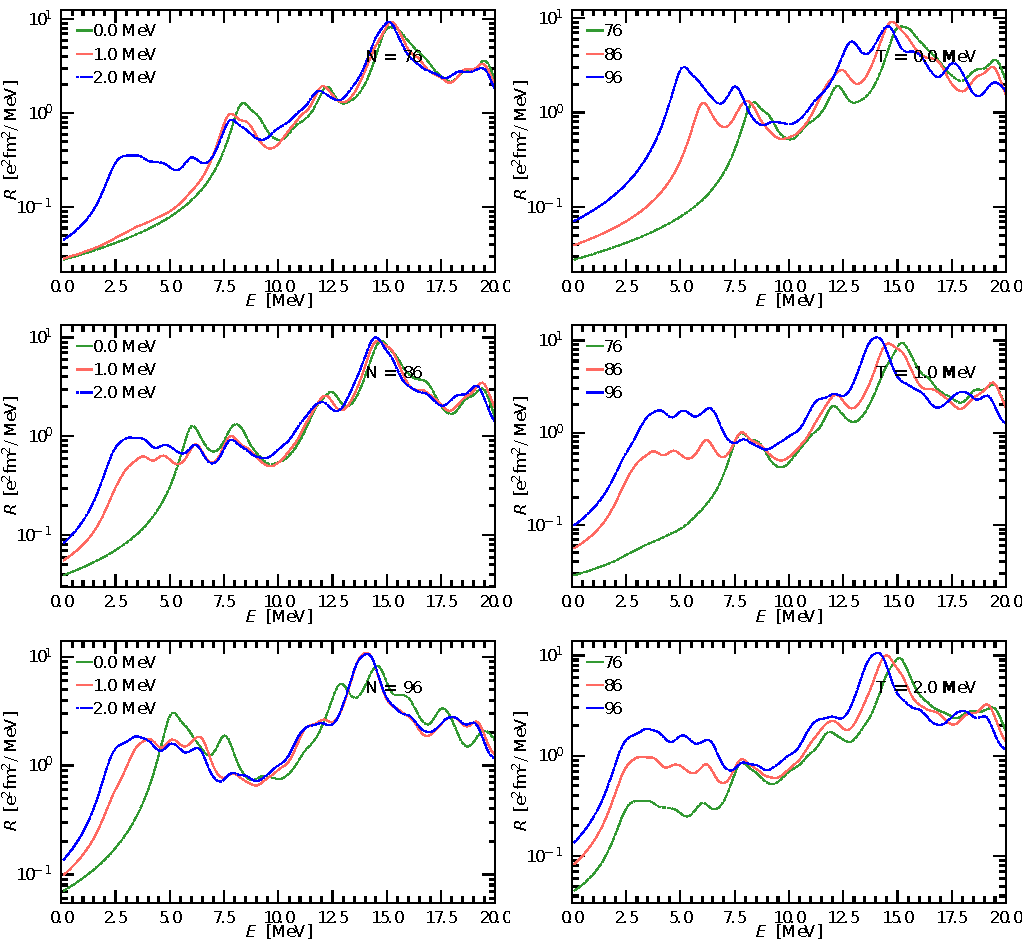
\includegraphics[width=0.4\textwidth]{images/photon_strength_function.pdf}
        \end{tikzfigure}
    }

    \block{~}{
	    Supported by ELI-NP Phase II, a project cofinanced by the 
	    Romanian Government and the EU through the European Regional Development
	    Fund and the Competitiveness Operational Program (1/07.07.2016,
	    COP, ID 1334)
        \begin{tikzfigure}
            
\includegraphics[width=0.2\textwidth]{images/three_logos.pdf}
        \end{tikzfigure}
	}
\end{columns}

\end{document}
